\documentclass{article}

\usepackage{amsmath}
\usepackage{float}
\usepackage{graphicx}
\usepackage{tikz}
\usepackage{textpos}

\usepackage[colorlinks=true, allcolors=blue]{hyperref}

\title{Lista 2}
\author{Luís Felipe Ramos Ferreira}
\date{\href{mailto:lframos.lf@gmail.com}{\texttt{lframos.lf@gmail.com}}
}

\begin{document}

\maketitle

\begin{itemize}
	\item (4.5.1)
		\begin{itemize}
			\item \(R(3)\)

				Inicialmente, note que a seguinte 2-coloração do \(K_5\) não possui uma clique de tamanho 3 monocromática, portanto
				\(R(3) > 5\). 

			                  \begin{figure}[H]
				                  \centering
				                  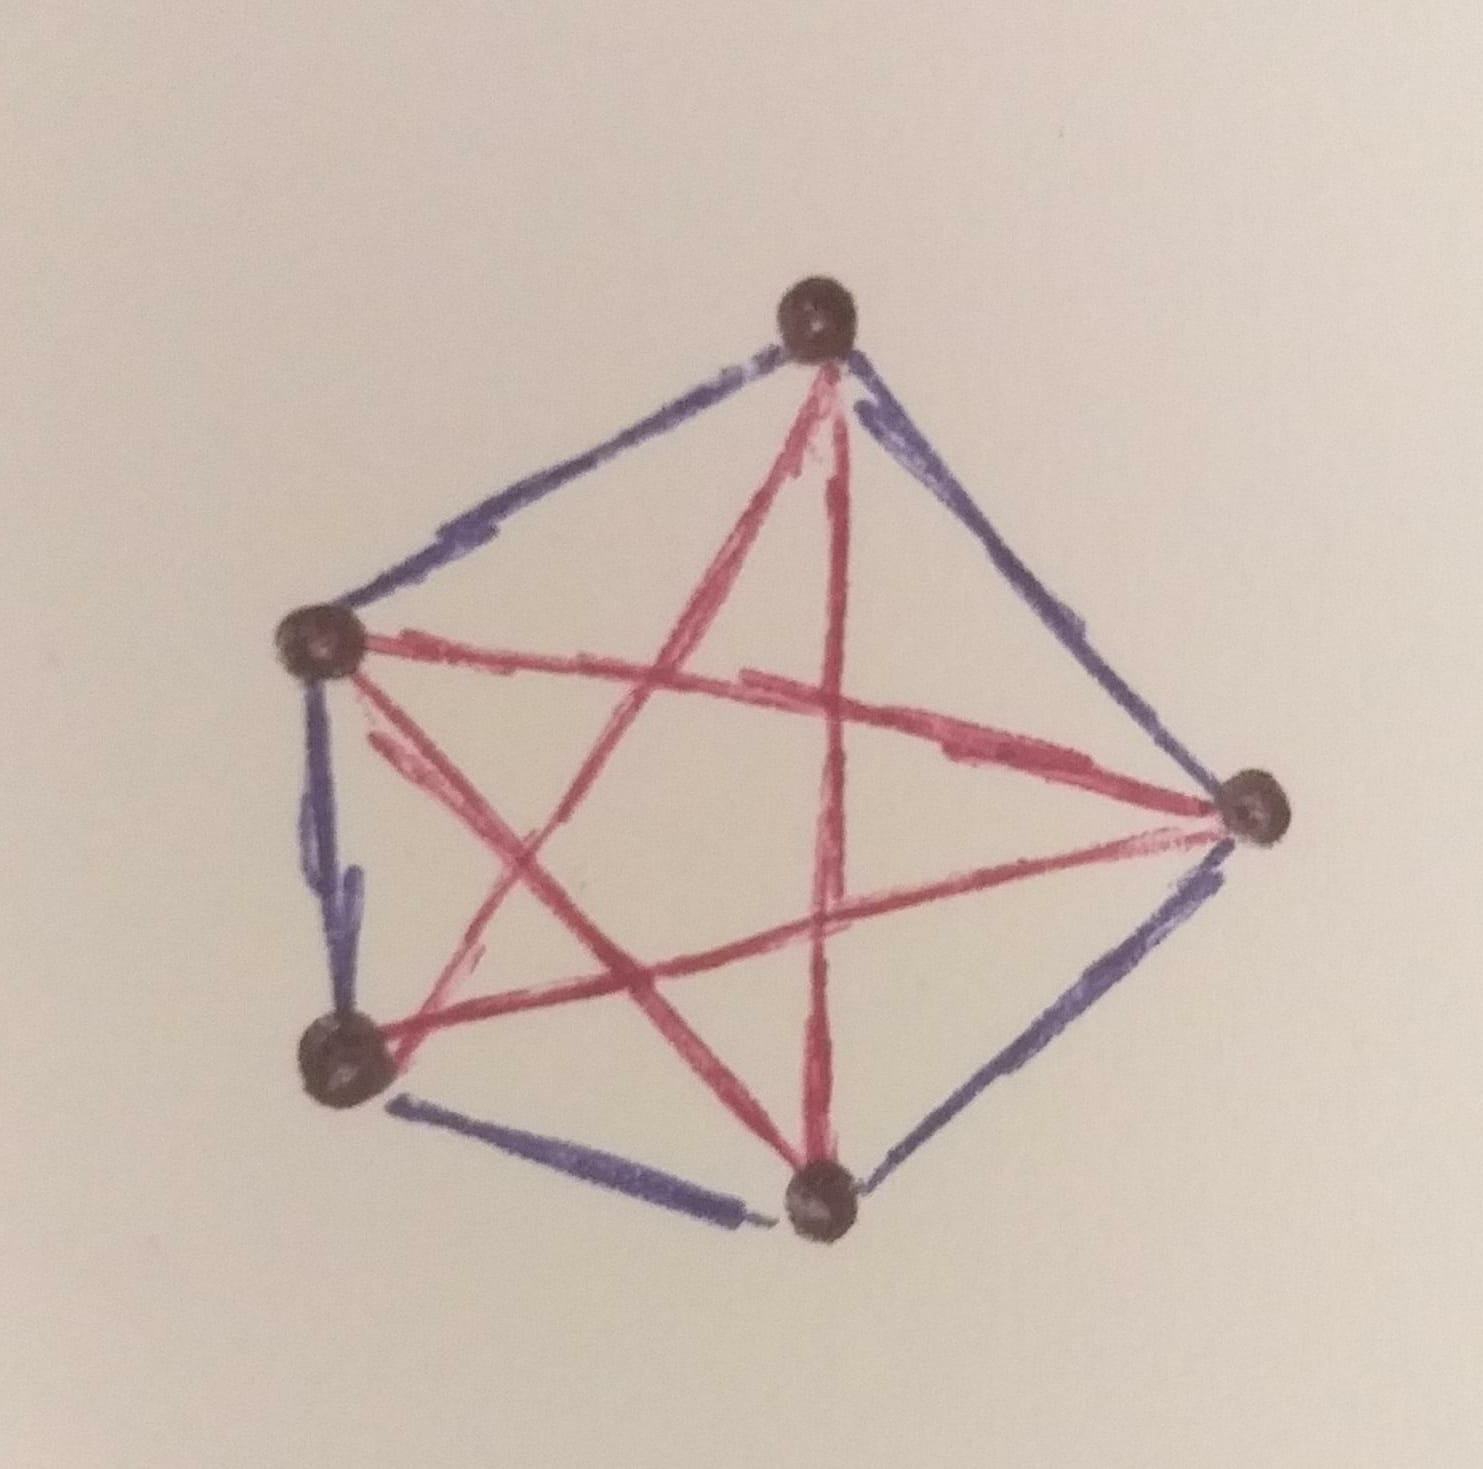
\includegraphics[width=0.8\textwidth]{images/1a.jpeg}
								  \caption{\(K_5\) 2-colorido}
			                  \end{figure}

				No entanto, sabemos pelo fato 4.0.1 do livro que o toda 2-coloração do \(K_6\) possui um triângulo monocromático, logo \(R(3) = 6\).
				A prova funciona da seguinte forma: seja \(v\) um vértice de \(K_6\). Pelo princípio da casa dos pombos, das 5 arestas incidentes a \(v\),
				ao menos 3 possuem a mesma cor. Vamos dizer que é a cor 1. Sejam \(x, y, z\) vizinhos de \(v\) com a aresta com cor 1. Se qualquer uma das arestas
				\(xy, xz, yz\) for da cor 1, temos um triângulo de cor 1. Caso contrário, o triângulo formado pelos vértices \(x, y, z\) é monocromático na outra cor,
				chamemos ela de 2. Logo, toda 2-coloração do \(K_6\) possui um triângulo monocromático.

			\item \(R(3, 4)\)

				Inicialmente, vamos notar que \(R(3, 4)\) é maior que 8, e isso pode ser notado pela 2-coloração do \(K_8\) abaixo em que
				não existe uma clique de tamanho 3 vermelha e nem uma clique de tamanho 4 azul (Na imagem, o primeiro grafo tem apenas as arestas vermelhas
				e o segundo seri ao complemento do primeiro grafo, em que as arestas são azuis).

			                  \begin{figure}[H]
				                  \centering
				                  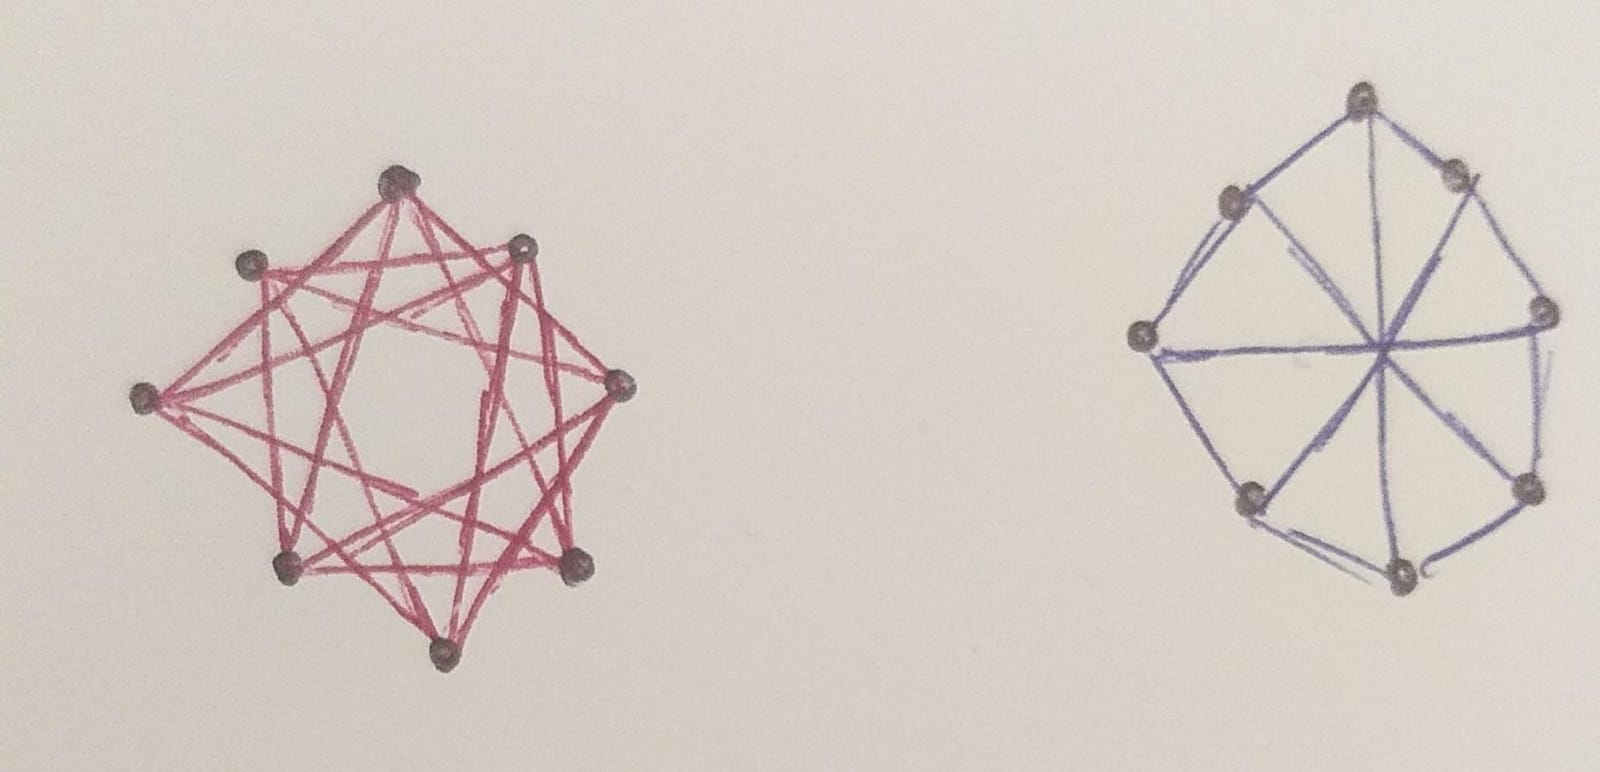
\includegraphics[width=0.8\textwidth]{images/1b.jpeg}
								  \caption{\(K_8\) 2-colorido}
			                  \end{figure}

				Vamos provar agora que \(R(3, 4) \leq 10\), em particular, mostrar que para um grafo completo de 10 vértices sempre teremos um triângulo
				vermelho ou uma clique de tamanho 4 azul. Depois, com uma pequena variação, mostraremos que \(R(3,4) \leq 9\), o que conclui a prova.

				Seja \(A\) um vértice qualquer de um \(K_{10}\) 2-colorido com vermelho e azul. \(A\) possui nove vizinhos e das arestas que o conectam a seus vizinhos,
				sabemos que ao menos 6 são azuis ou ao menos 4 são vermelhas (isso porque no total precisamos ter 9 arestas, uma para cada vizinho). Suponhamos o caso em que
				\(A\) possui 4 arestas vermelhas o conectando a seus vizinhos. Se existir uma aresta vermelha entre esses vizinhos, então existe um triângulo vermelho no grafo. Caso
				contrário, todas as arestas entre os 4 vértices são azuis, logo existe uma clique de tamanho 4 de cor azul. Seja agora o caso em que \(A\) possui
				6 arestas de cor azul o conectando a seus vizinhos. Sabemos que \(R(3, 3) = 6\), logo, entre esses vizinhos, há um triângulo vermelhor ou azul. Se for vermelho,
				já perdemos, se for azul, note que ele forma uma clique de tamanho 4 azul junto com \(A\). Logo, \(10\) é um limite superior para \(R(3, 4)\).
				
				Consideremos agora o caso do \(K_9\). Note que os argumentos usados anteriormente servem da mesma maneira, exceto pelo caso em que, para todo vértice \(A\),
				exista exatamente 5 arestas azuis e 3 vermelhas saindo dele. Nesse caso, para cada vértice teremos três arestas vermelhas, e como são 9 vértices, temos \(3 * 9 = 27\). Como cada arestas
				é contada duas vezes, precisamos dividir por dois, obtendo assim um número \(\frac{27}{2}\)(não inteiro) de arestas, o que é um absurdo. Logo, \(R(3, 4) \leq 9\)

			\item \(R(4, 4)\)

				Sabemos pelo lema 4.1.3 do livro que, para todo \(s, t \geq 2\), temos:
				\[R(s, t) \leq R(s - 1, t) + R(s, t - 1)\]

				Logo, temos que \(R(4, 4) \leq R(3, 4) + R(4, 3) = 2*R(3, 4) = 2*9 = 18\)
				No entanto, vamos mostrar que existe uma 2-coloração de \(K_{17}\) tal que não existe uma clique de tamanho 4 nem vermelha nem azul, mostrando assim
				que \(R(4, 4) = 18\). Como um grafo de 17 vérticesé muito grande para ser desenhado, vamos fazer uma construção analitica dele. Seja um \(K_{17}\) e vamos
				2-colorir suas arestas da seguinte forma:



				\end{itemize}

			\item (4.5.2)
			\item (4.5.3)
			\item (4.5.4)
			\item (4.5.5)
			\item (4.5.6)
			\item (4.5.7)
			\item (4.5.8) OPCIONAL
			\item (4.5.9)
			\item (4.5.10)
		\end{itemize}

	\end{document}
